\section*{\centering IMAGE RECOGNITION–BASED MONGOLIAN SCRIPT LEARNING APPLICATION}

\begin{flushright}
\deptname\\
Student: \authorcode, \authorshort\\
Supervisor: \supervisor
\end{flushright}


\setcounter{section}{0}
\renewcommand{\thesection}{\arabic{section}}
\titleformat{\section}
  {\normalfont\normalsize\bfseries}
  {\thesection.}
  {0.4em}
  {}

\begin{multicols}{2}

\section*{Introduction}
Mongolian script is an important part of Mongolia’s history, culture, and national identity. However, in modern society, Cyrillic script is used more widely, so learning and practicing Mongolian script has become less common. For many young people, it is difficult to find a simple and engaging way to study regularly.

In recent years, mobile technology has created new opportunities for education. Mobile applications allow users to learn anytime and anywhere, in short sessions, and track their progress easily. Because of this, digital learning tools are becoming more popular and effective.

Based on this need, the Egüü app was developed. This application helps users learn Mongolian script step by step on mobile devices. It is not only focused on memorizing letters, but also on tracking user progress and supporting daily learning habits.

The app is built using React Native, Firebase, and TensorFlow.js. These technologies allow the system to run on both iOS and Android, store data in the cloud, and support handwriting recognition. Therefore, this project combines traditional language learning with modern technology.

\section*{Goal}
The main goal of this project is to make learning Mongolian script easier, more accessible, and more effective using modern technology. The system is designed not only to provide content, but also to guide users based on their learning progress.

Another important goal is to solve common problems such as irregular practice, low motivation, and the difficulty of checking handwritten characters. The Egüü app aims to help users build a daily learning habit and improve gradually.

\section*{Objectives}
To achieve this goal, the following objectives were defined:
\begin{enumerate}
    \item Develop a mobile application for learning Mongolian script
    \item Implement a flashcard system for repetition
    \item Use OCR to recognize handwritten characters
    \item Store user progress and statistics
    \item Use Firebase for authentication and data storage
    \item Support both Mongolian and English languages
    \item Create a system that can be expanded in the future
\end{enumerate}

These objectives focus not only on technical implementation, but also on user experience and long-term system scalability.

\section*{Methodology}
The system was developed using a cross-platform approach with React Native. This allows one codebase to run on both iOS and Android devices, making development faster and easier to maintain.

Firebase was used as the backend system. Firebase Authentication manages user login and security, while Firestore stores data such as letters, flashcards, user progress, and settings. Offline support allows users to continue learning even without internet access.

The main system functions are illustrated in the use case diagram.

\begin{center}
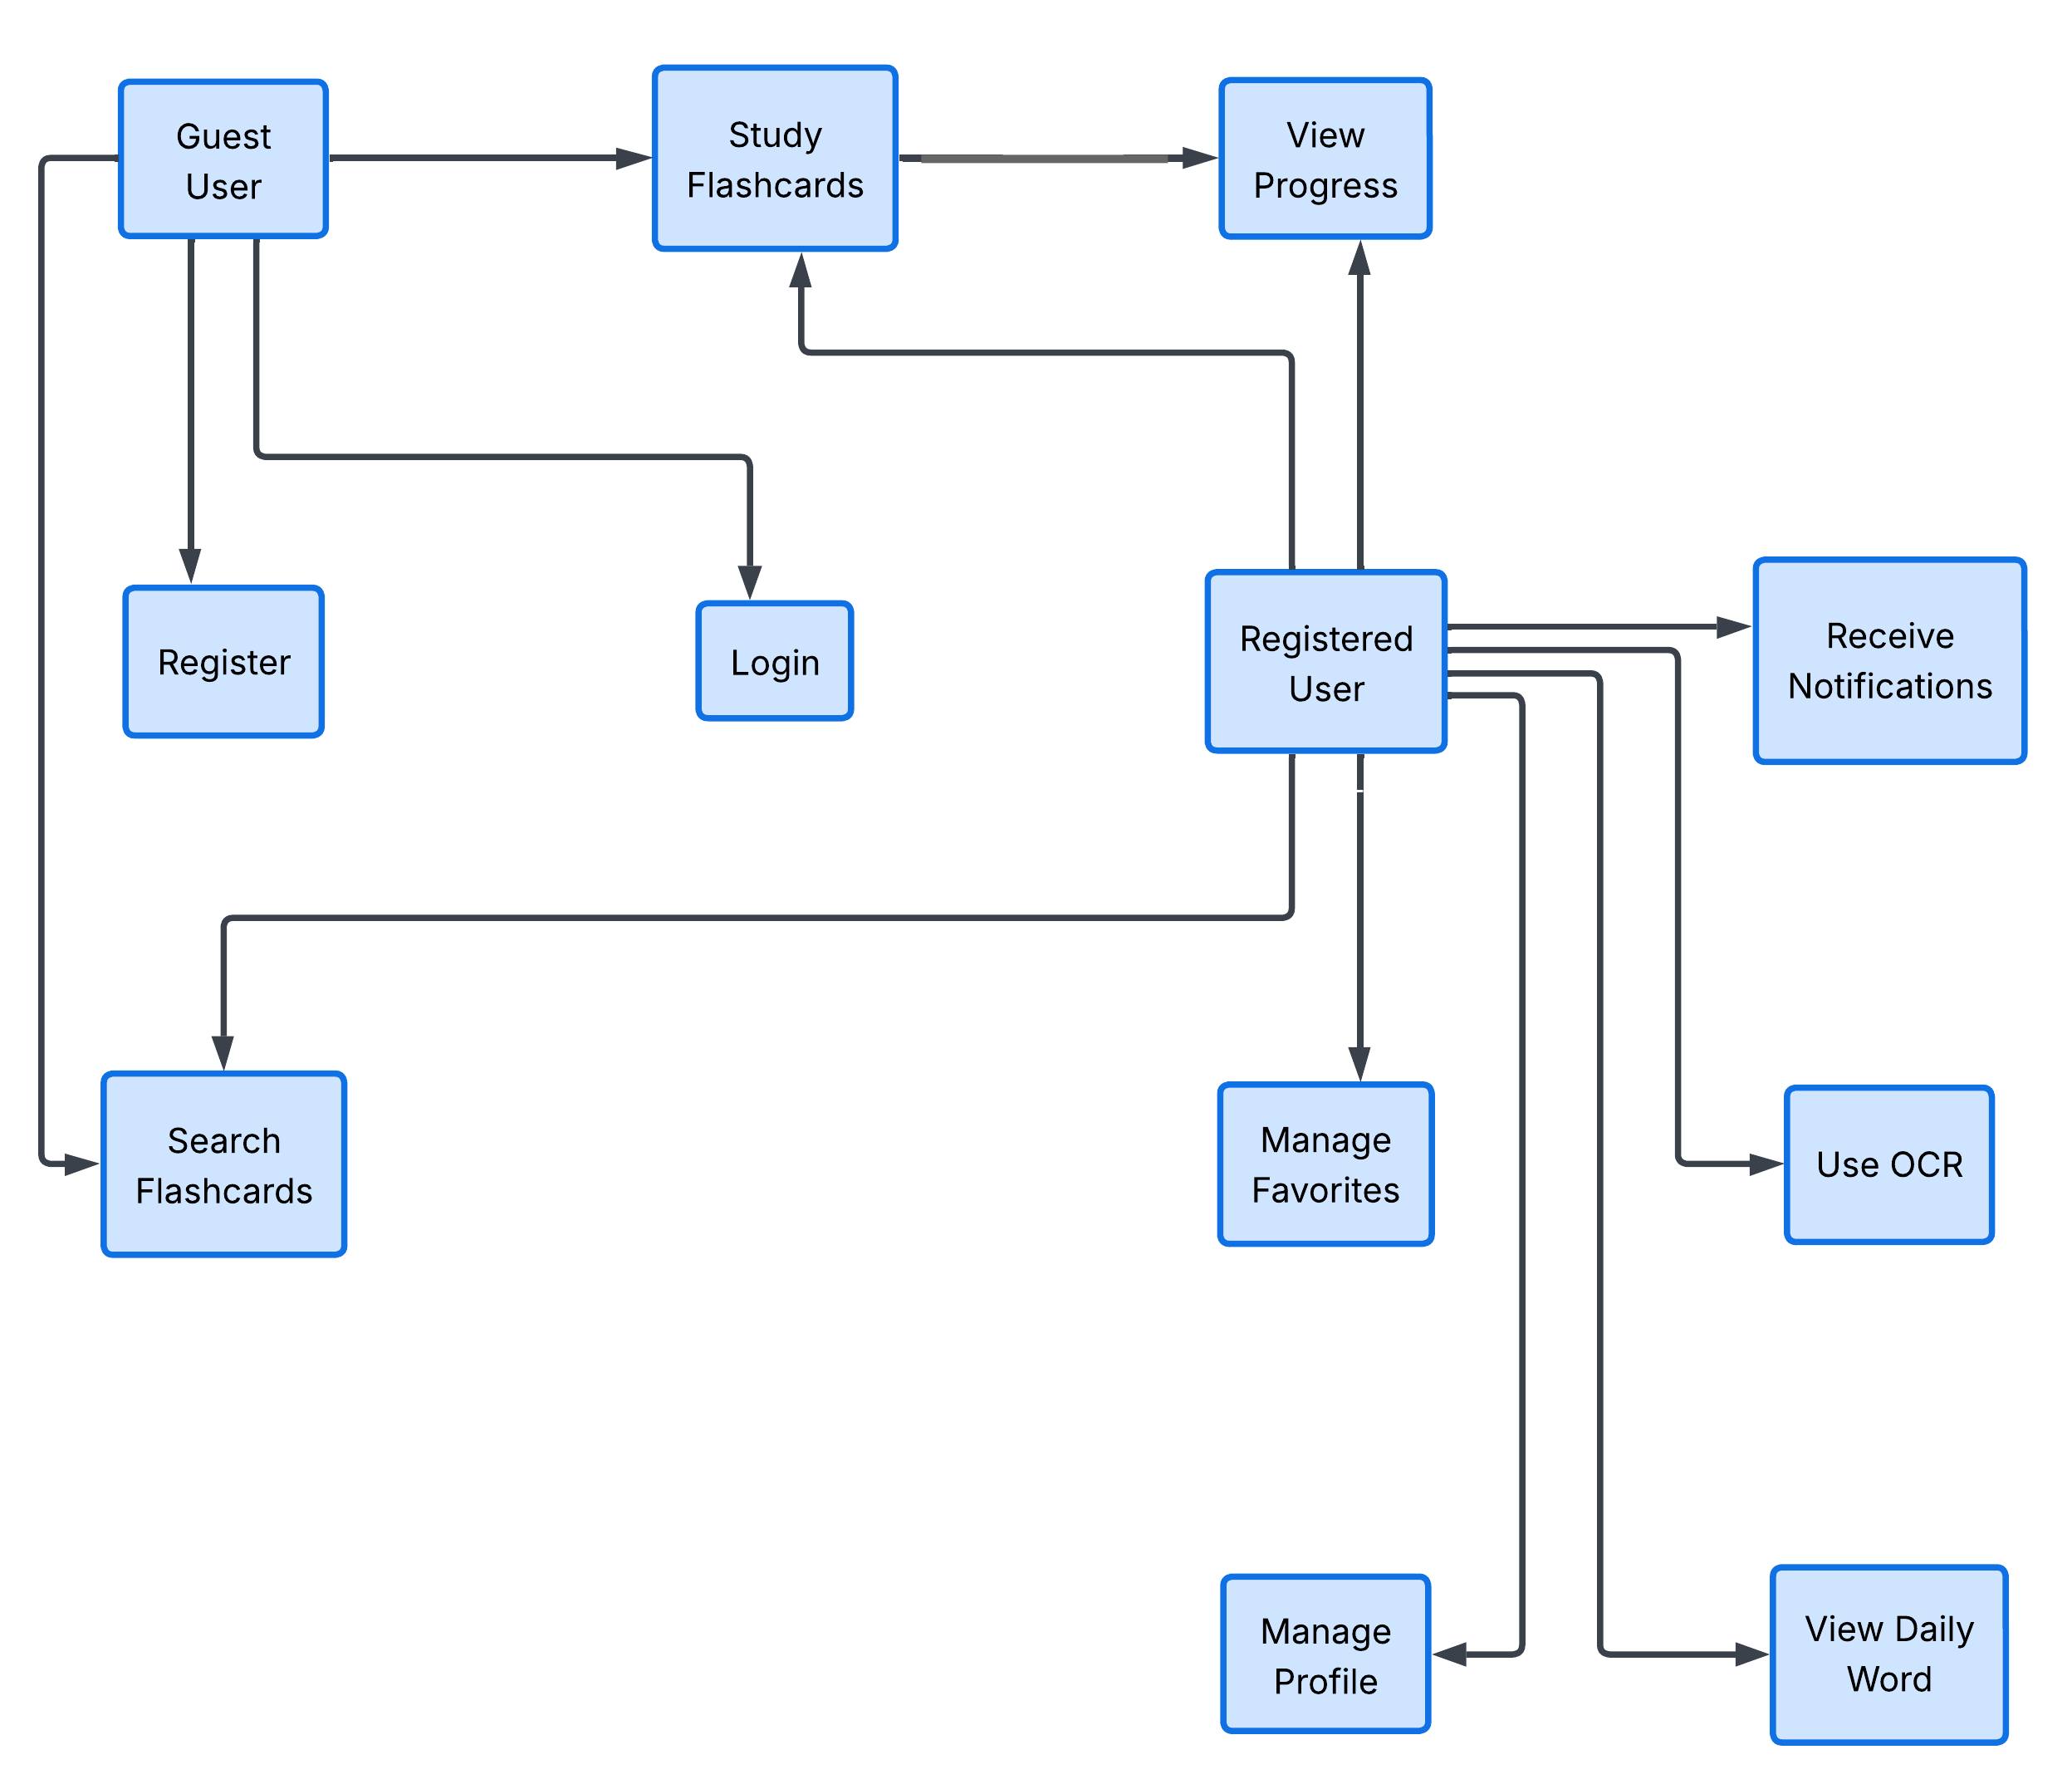
\includegraphics[width=0.68\columnwidth]{Figures/diagrams/usecasediagram.png}
\footnotesize
\captionof{figure}{Use case diagram of the system}
\end{center}

\vspace{-6pt}
The data flow diagram shows how data moves between the user, the application, and the database. For example, when a user answers a flashcard, the result is saved in Firestore and used for future repetition logic.

\begin{center}
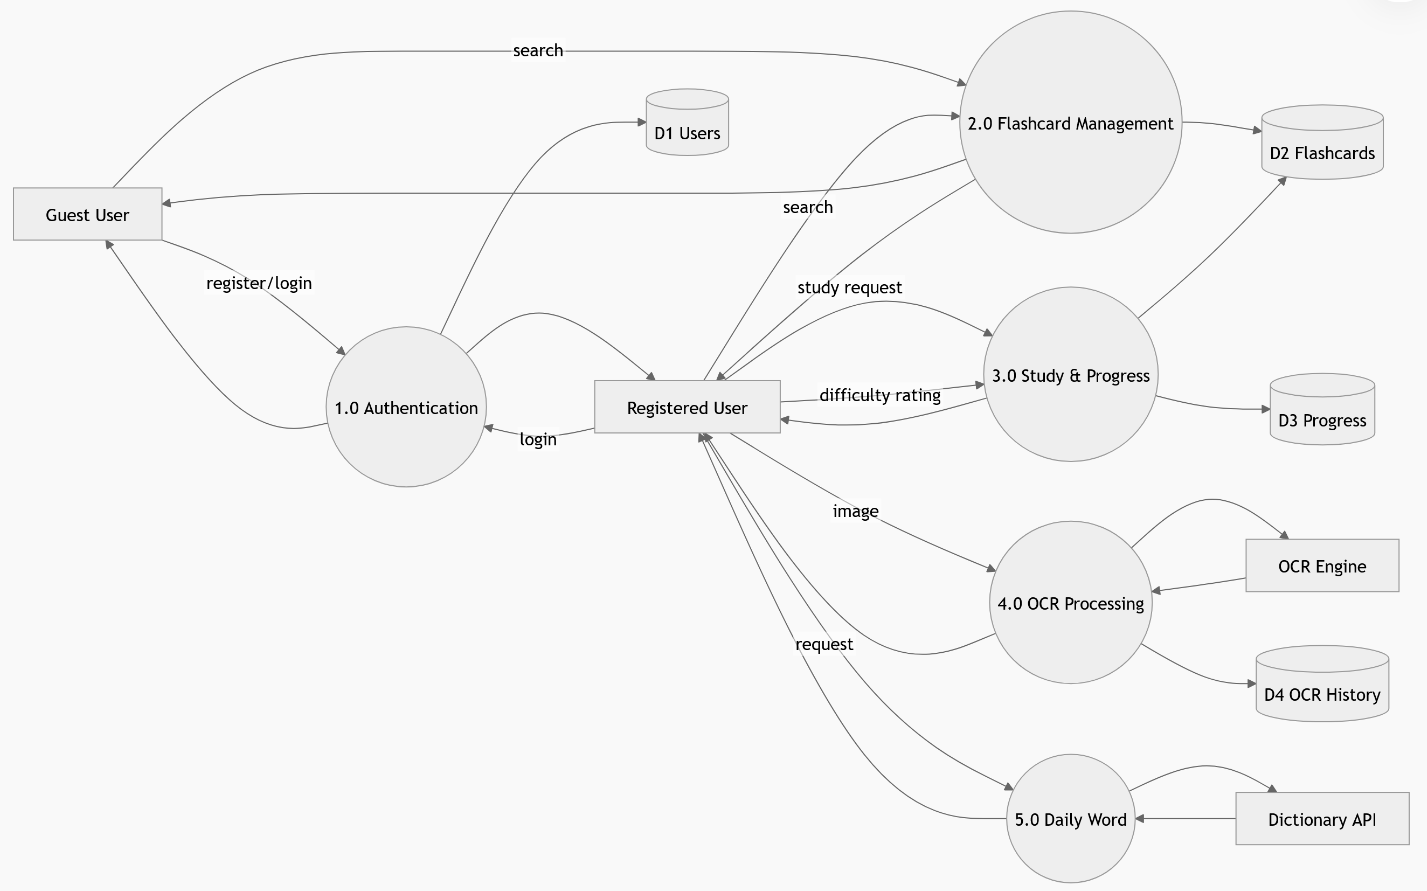
\includegraphics[width=0.68\columnwidth]{Figures/diagrams/dataflow.png}
\footnotesize
\captionof{figure}{Data flow diagram of the system}
\end{center}

\vspace{-6pt}
For OCR, TensorFlow.js was used. Input images are processed into 28×28 grayscale format and then classified by the model. This allows users to write characters and get instant feedback.

\begin{center}
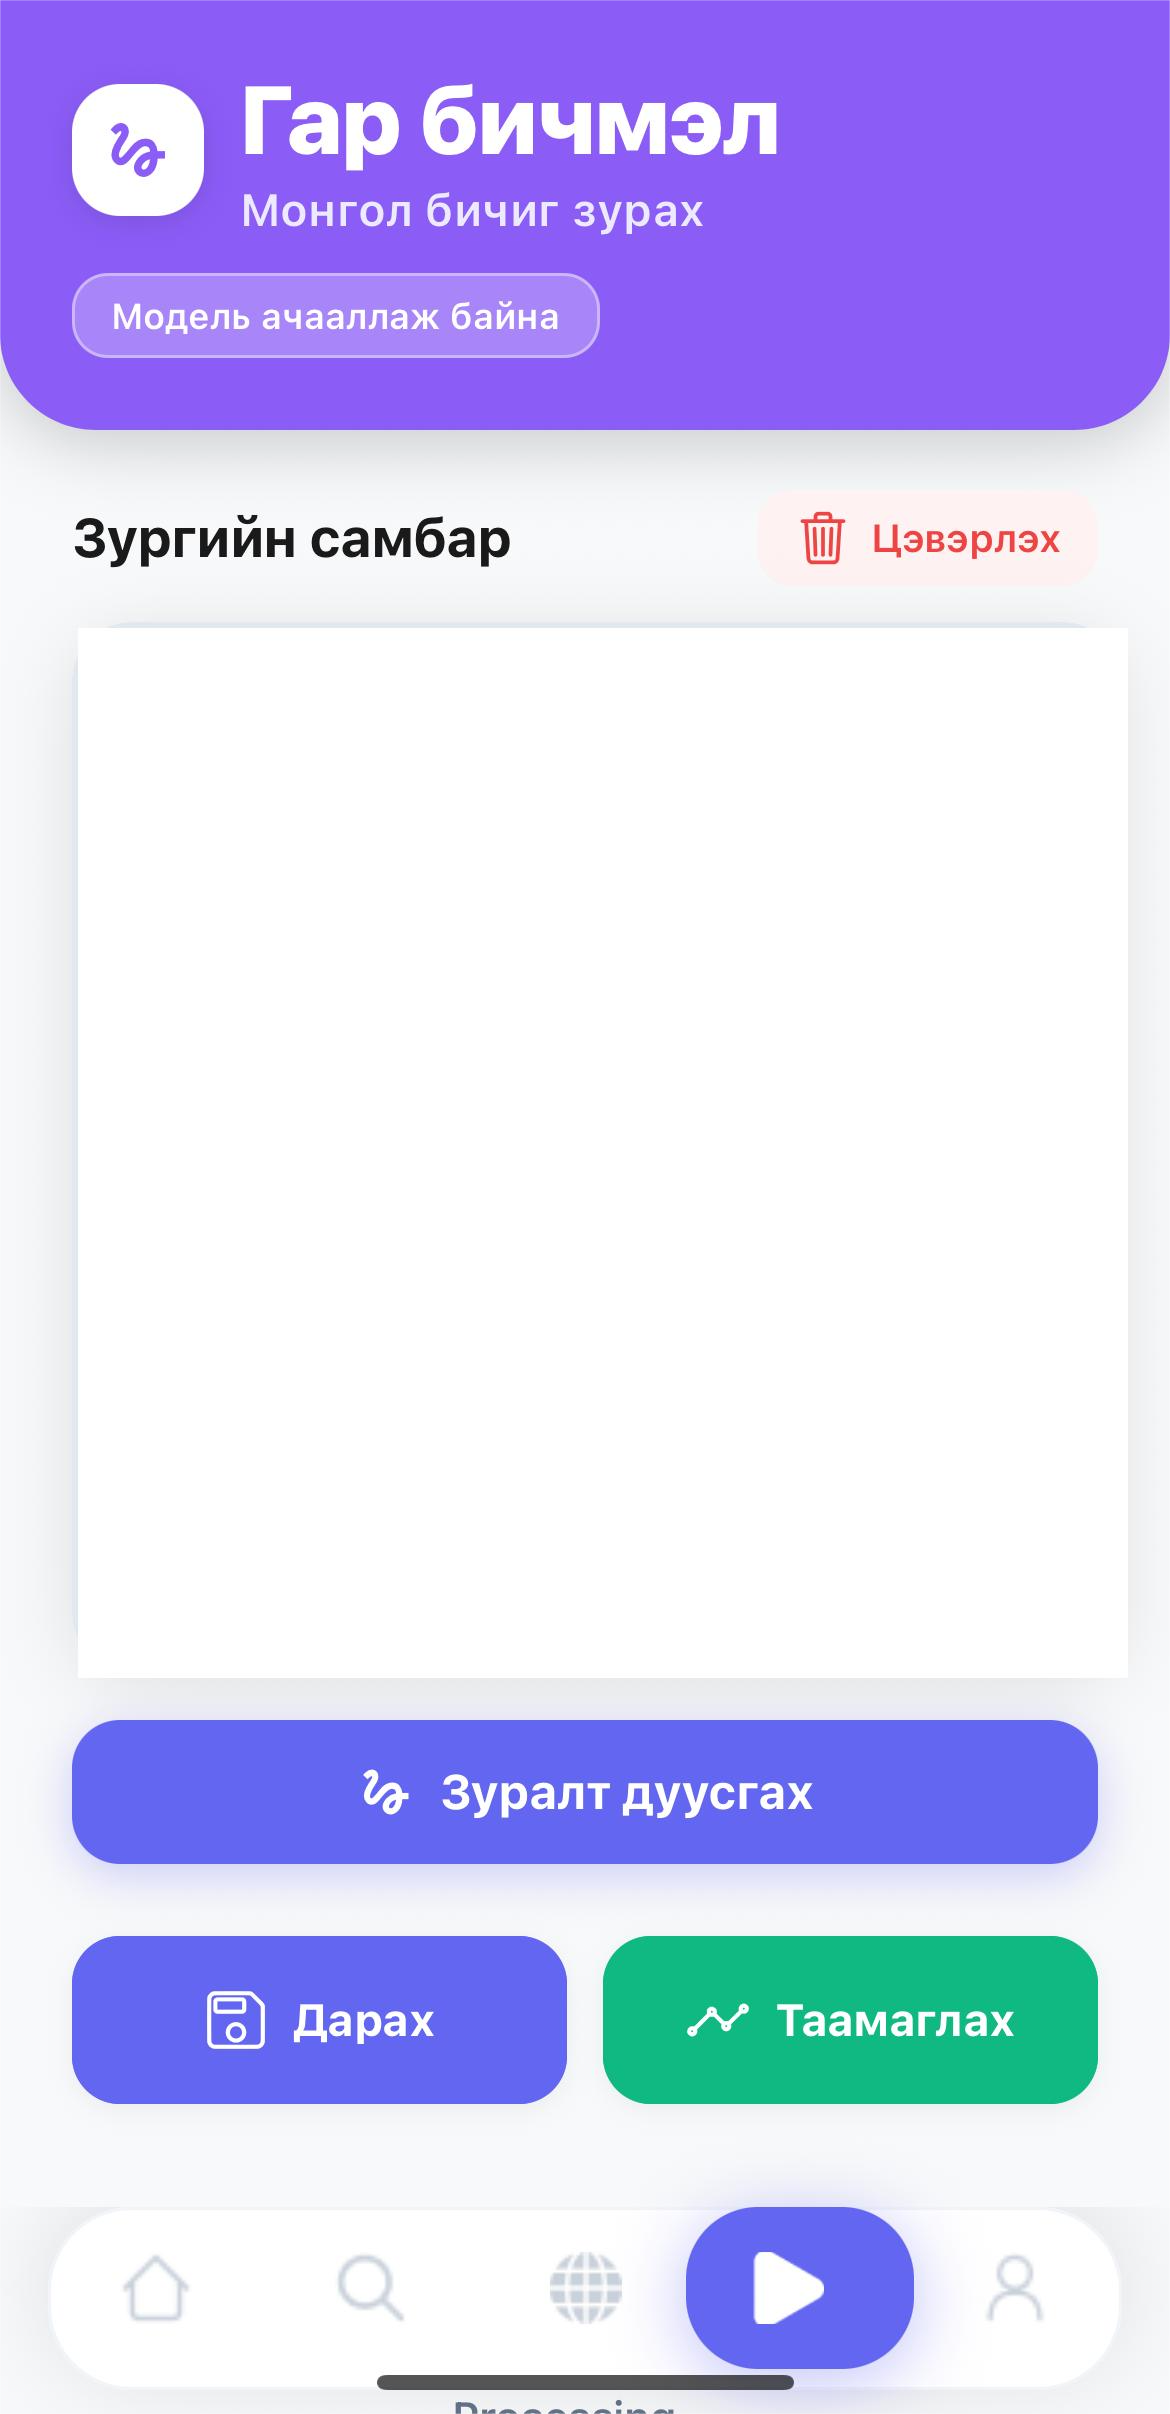
\includegraphics[width=0.62\columnwidth]{Figures/pages/handwriting.png}
\footnotesize
\captionof{figure}{Handwriting input interface}
\end{center}

\section*{Results}
After implementation, the system was evaluated based on several requirements. Most of the planned features were successfully completed.

\begin{center}
\captionof{table}{System results}
\small
\resizebox{\columnwidth}{!}{
\begin{tabular}{|l|l|l|}
\hline
Criteria & Goal & Result \\
\hline
Platform & iOS + Android & Completed \\
Flashcards & 500+ & 520 \\
Categories & 5+ & 7 \\
Language & 2 & Mongolian, English \\
Theme & Dark/Light & Completed \\
OCR & Mongolian script & Basic letters recognized \\
Offline & Supported & Firestore used \\
\hline
\end{tabular}}
\end{center}

The OCR model performance is shown below:

\begin{itemize}
    \item Training accuracy: 92\%
    \item Validation accuracy: 87\%
    \item Test accuracy: 85\%
    \item CER: 15\%
    \item WER: 28\%
\end{itemize}

The model performs well on character recognition, but errors are higher at the word level. This may be caused by similar-looking characters and limited data diversity.

\begin{center}
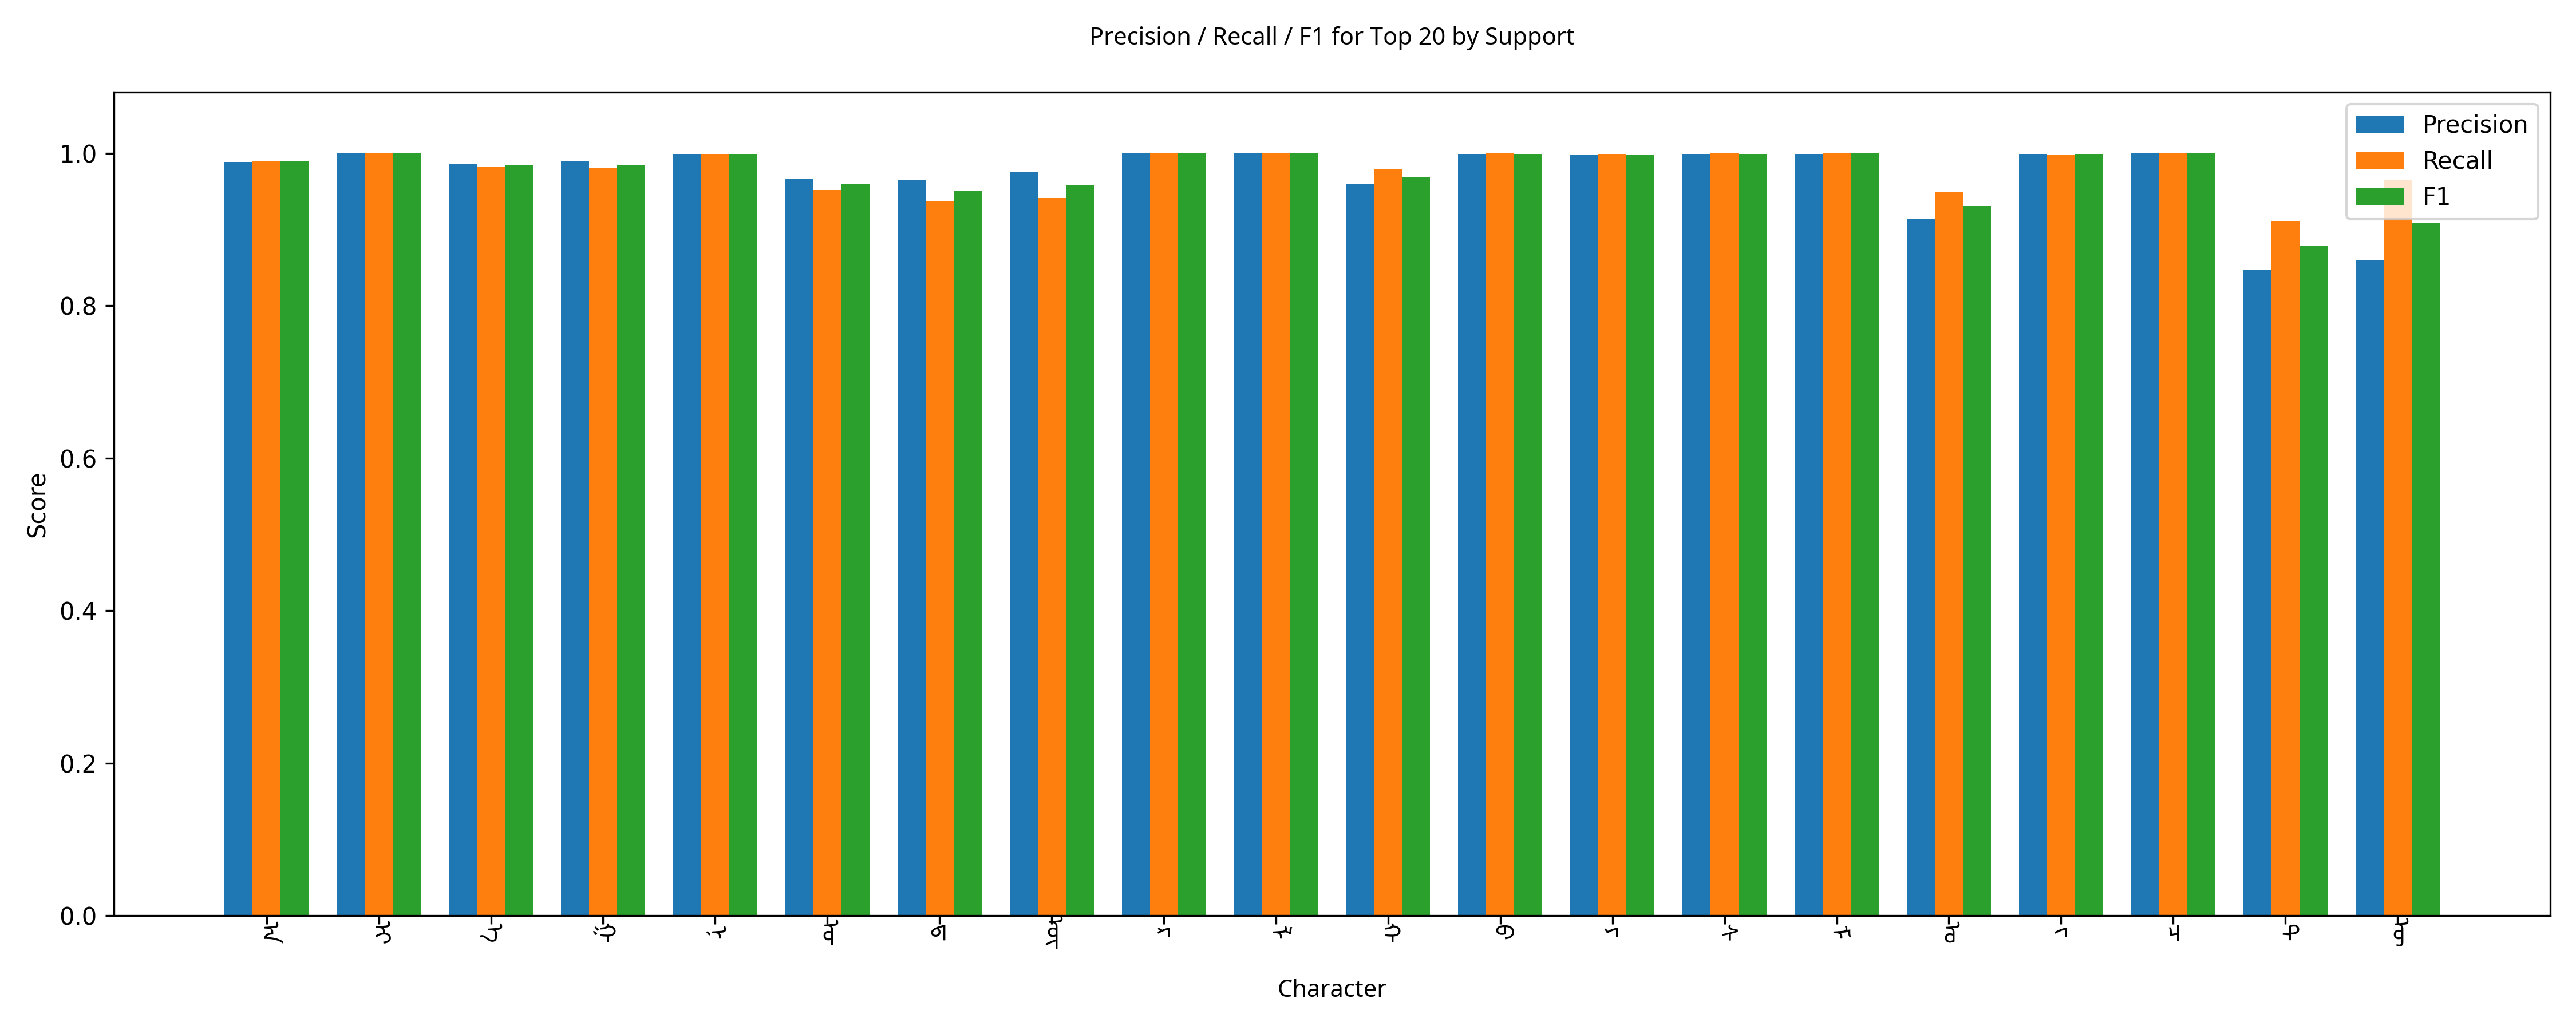
\includegraphics[width=0.66\columnwidth]{Figures/evalution/prf_top_support_clean.png}
\footnotesize
\captionof{figure}{Precision, recall, and F1 score of OCR model}
\end{center}

The dataset used for training is shown below.

\begin{center}
\captionof{table}{OCR dataset}
\small
\begin{tabular}{|l|r|}
\hline
Training data & 40000 \\
Validation data & 9615 \\
Test data & 20000 \\
Total & 69615 \\
\hline
\end{tabular}
\end{center}

\section*{Conclusion}
In this project, the Egüü app was successfully developed as a Mongolian script learning system. The system supports cross-platform usage, secure data storage, and OCR-based handwriting recognition.

By combining flashcards, OCR, and user progress tracking, the app provides a more flexible and effective learning experience. Firebase also allows centralized data management and personalized learning.

The results show that this system has strong potential for real-world educational use. In the future, improvements can include increasing OCR accuracy, adding adaptive learning algorithms, and introducing gamification features.

\section*{References}
\printbibliography[heading=none]

\end{multicols}
